\documentclass[hyperref={pdfpagelabels=false}]{beamer}
% Die Hyperref Option hyperref={pdfpagelabels=false} verhindert die Warnung:
% Package hyperref Warning: Option `pdfpagelabels' is turned off
% (hyperref)                because \thepage is undefined. 
% Hyperref stopped early 
%

\usetheme{Heidelberg}
\usepackage{wrapfig}
\usepackage{lmodern}

\usepackage{natbib}
\usepackage{amsmath,amsfonts,amssymb}

\usepackage{algorithm,algorithmic}

\usepackage{tikz}
	\usetikzlibrary[topaths,arrows,calc]
\usepackage{wrapfig}



\usepackage[ngerman]{babel}
\usepackage[T1]{fontenc} % Ligaturen, richtige Umlaute im PDF 
\usepackage[utf8]{inputenc}% UTF8-Kodierung für Umlaute usw

\usepackage{hyperref}

\definecolor{darkred}{rgb}{110,1,1}  
\definecolor{maroon}{rgb}{0.5,0,0}  

\newcounter{saveenumi}
\newcommand{\seti}{\setcounter{saveenumi}{\value{enumi}}}
\newcommand{\conti}{\setcounter{enumi}{\value{saveenumi}}}


% Wenn \titel{\ldots} \author{\ldots} erst nach \begin{document} kommen,
% kommt folgende Warnung:
% Package hyperref Warning: Option `pdfauthor' has already been used,
% (hyperref) ... 
% Daher steht es hier vor \begin{document}

\title{{\textcolor{red}H}yperlink {\textcolor{red}I}nduced
	   {\textcolor{red}T}opic {\textcolor{red}S}earch (HITS)}   
\author{Ekaterina Tikhoncheva\\
		\vspace{20pt}
		Seminar \glqq Information Retrieval\grqq\\} 
\date{Universität Heidelberg\\19.01.2014} 

% zusaetzlich ist das usepackage{beamerthemeshadow} eingebunden 
\usepackage{beamerthemeshadow}

%\usepackage{filecontents}
%\usepackage[style=chem-angew]{biblatex}

%  \beamersetuncovermixins{\opaqueness<1>{25}}{\opaqueness<2->{15}}
%  sorgt dafuer das die Elemente die erst noch (zukuenftig) kommen 
%  nur schwach angedeutet erscheinen 
%\beamersetuncovermixins{\opaqueness<1>{25}}{\opaqueness<2->{15}}
% klappt auch bei Tabellen, wenn teTeX verwendet wird\ldots
\begin{document}

%                               Inhaltsverzeichnis                                           %
\begin{frame}
\titlepage
\end{frame}
%--------------------------------------------------------------------------%
\begin{frame}
\frametitle{Agenda}
\tableofcontents
\end{frame} 

%--------------------------------------------------------------------------%
\section{Einführung} 
\begin{frame}
\frametitle{Einführung}

\begin{itemize}
\item HITS ist ein Algorithmus zum Finden und Bestimmen der Rangordnung der zu einer gegebenen Suchanfrage relevanten Seiten im WWW\footnote{in einer Hyperlinked-Umgebung}

\item Entwickelt von Jon M. Kleinberg, 1997 IBM Research Report RJ 10076

\item Idee: finde autoritäre Informationsquellen (engl. {\bf authorities}) zu der gegebenen Suchanfrage

\item Mathematischer Hintergrund: Eigenvektoren der mit dem Web-Graphen verbundenen Matrix  
\end{itemize}

\end{frame}


%--------------------------------------------------------------------------%
\section{Grundidee} 
\begin{frame}
\frametitle{Drei Typen der Suchanfragen}
\begin{itemize}
\item spezielle: \hspace{50pt}
						\visible<2->{\textcolor{red}{Problem der Knappheit}} \\
	\glqq Does Netscape support the JDK 1.1 - code-signing API?\grqq
	\cite{Kleinberg}
	\begin{block}{}
	\item 
	breit angelegte: \hspace{30pt} 	
					\visible<3->{\textcolor{red}{Problem der Vielfältigkeit}} \\
	\glqq Find information about the Java programming language\grqq \cite{Kleinberg}
	\end{block}
	
	\item Suche nach ähnlichen Seiten\\
	\glqq Find pages similar to {\it java.sun.com}\grqq\cite{Kleinberg}
	
\end{itemize}
\end{frame}

\begin{frame}
\frametitle{Ranking}

\begin{itemize}
\item Man möchte die meist relevanten und nützlichen Seiten (Autoritätsseiten) aus der Menge aller zu der Anfrage relevanten Seiten finden
\item Mögliche Hindernisse:
	\begin{itemize}
	\item die meist relevanten Seiten werden nicht unbedingt durch ein textbasiertes Ranking vorgezogen
	\item es kann sein,  dass die relevanten Seiten die Wörter aus der Suchanfrage gar nicht enthalten
	\end{itemize}
\end{itemize}
\end{frame}


\begin{frame}[allowframebreaks]

\begin{block}{Annahme}
Die Relevanz zwischen zwei Seiten wurde vom Ersteller des Links zwischen diesen Seiten geprüft
\end{block}

Stimmt im Allgemeinen nicht (z.B. Navigationslinks, Werbung)
\vspace{10pt}

Aber unter dieser Annahme reicht es nur die Linkstruktur des WWW zu betrachten, um die Autorität einer Seite im Bezug auf eine andere zu bestimmen

\frametitle{Authorities und Hubs}

\framebreak

\begin{block}{Authorities (Autoritätsseiten)}
Relevante Seiten, auf die viele weitere relevante Seiten zeigen
\end{block}

\vspace{5pt}
\begin{minipage}[0.2\textheight]{\textwidth}
	\begin{columns}[T]
		\begin{column}{0.7\textwidth}
			{\bf Problem}: populäre Seiten kommen immer als Authorities vor
			
			\vspace{10pt}
			Es muss eine Überlappung in den Links, die auf Authorities zeigen, berücksichtigt werden
		\end{column}
		\begin{column}{0.2\textwidth}
			\begin{figure}
			\begin{tikzpicture}
				\node[] (h) at ( 1.0, 1.3) {Hubs};
				\node[] (v3) at ( 0.0, 0.0) {};\fill[red] (v3) circle (2pt);
				\node[] (v4) at ( 1.0, 0.0) {};\fill[red] (v4) circle (2pt);
				\node[] (v5) at ( 2.0, 0.0) {};\fill[red] (v5) circle (2pt);
			
				\node[] (v0) at ( 0.0, 1.0) {};\fill[blue] (v0) circle (2pt);
				\node[] (v1) at ( 1.0, 1.0) {};\fill[blue] (v1) circle (2pt);
				\node[] (v2) at ( 2.0, 1.0) {};\fill[blue] (v2) circle (2pt);
				
				\draw[->] (v2) to node[right] {} (v4);
				
				\draw[->] (v0) to node[right] {} (v3);
				\draw[->] (v0) to node[right] {} (v5);
				
				\draw[->] (v1) to node[right] {} (v3);
				\draw[->] (v1) to node[right] {} (v4);
				
				\node[] (a) at ( 1.0, -.2) {Authorities};
			\end{tikzpicture}
			\end{figure}
		\end{column}
	\end{columns}
\end{minipage}

\begin{block}{Hubs}
Seiten, die auf viele Authorities zeigen
\end{block}

\end{frame}


%--------------------------------------------------------------------------%
\section{Algorithmus}

\begin{frame}
\frametitle{HITS Algorithmus}
Der Algorithmus besteht aus zwei Schritten:
\begin{enumerate}
\item Konstruiere einen auf die Suchanfrage fokussierten Teilgraphen des WWW 
\item Berechne rekursiv die Authorities- und Hubgewichte für alle Knoten im Teilgraphen aus Schritt 1
\end{enumerate}

\end{frame}


\subsection{Schritt $1$} 
\begin{frame}
\frametitle{Teilgraph vom WWW}
Wir stellen das ganze Web als ein gerichteter Graph $G=(V,E)$ dar. Gesucht wird ein auf der Anfrage basierter Teilgraph vom WWW

\vspace{10pt}
Sei eine Suchanfrage $\sigma$ gegeben. Wir bezeichnen mit $\mathbf{Q_\sigma}$ das Ergebnis der textbasierten Suche
\begin{itemize}
\item $Q_\sigma$ ist groß
\item Gute Authorities müssen nicht in $Q_\sigma$ liegen
\end{itemize}

\vspace{10pt}

Gesucht wird eine Menge $\mathbf{S_\sigma}$ von Seiten, die
\begin{itemize}
\item klein ist
\item relevante Seiten enthält
\item viel gute Authorities enthält 
\end{itemize}
\end{frame}


\begin{frame}

\begin{minipage}[0.2\textheight]{\textwidth}
	\begin{columns}[T]
		\begin{column}{0.6\textwidth}

			\begin{algorithm}[H]
				\begin{algorithmic}[1]
				
				\STATE $R_\sigma$ ist die Menge der $t$ besten Ergebnisse\\
						des textbasierten Suchalgorithmus $E$\\
						angewendet auf die Anfrage (engl. {\bf root set}) $\sigma$
				\STATE $S_\sigma:=R_\sigma$
				\FOR{$p$ in $R_\sigma$}
				\STATE $S_\sigma = S_\sigma \cup \{Menge\ der\ Seiten,\ auf\ die\ $p$\ zeigt \} $ \STATE $S_\sigma = S_\sigma \cup \{Menge\ der\ $d$\ Seiten,\ die\ auf\ $p$\ zeigen \}$
				\ENDFOR
				\end{algorithmic}
				\caption{Teilgraphen($\sigma$, $E$, $t$, $d$) }

			\end{algorithm}

		\end{column}
	\begin{column}{0.3\textwidth}
		\begin{figure}
		\vbox{ \begin{tikzpicture}
			\filldraw[red!45] (0.3, 0.2) ellipse(1cm and 0.8 cm);
			
			\node[] (v1) at ( 0.0, 0.0) {};\fill (v1) circle (2pt);
			\node[] (v2) at ( 0.0, 0.5) {};\fill (v2) circle (2pt);
			\node[] (v3) at ( 0.8, 0.2) {};\fill (v3) circle (2pt);
			
			\node[] (v4) at (-1.0, 2.5) {};\fill (v4) circle (2pt);
			\node[] (v5) at ( 1.5, 3.0) {};\fill (v5) circle (2pt);
			
			\node[] (v6) at (-1.7, 0.8) {};\fill (v6) circle (2pt);
			
			\node[] (v7) at ( 2.0, 0.8) {};\fill (v7) circle (2pt);
			
			\node[] (v8) at (-0.7,-1.0) {};\fill (v8) circle (2pt);
			\node[] (v9) at ( 1.3,-1.5) {};\fill (v9) circle (2pt);
			
			\draw[->] (v2) to node[right] {} (v3);
			
			\draw[->, thick, blue] (v2) to node[right] {} (v6);
			\draw[->, thick, green] (v4) to node[right] {} (v2);
			\draw[->, thick, blue] (v3) to node[right] {} (v5);
			\draw[->] (v4) to node[right] {} (v5);
			
			\draw[->, thick, green] (v6) to node[right] {} (v1);
			
			\draw[->, thick, blue] (v3) to node[right] {} (v7);
			
			\draw[->, thick, green] (v8) to node[right] {} (v1);
			\draw[->] (v8) to node[right] {} (v9);
			
			\draw (0.3, 1.0) ellipse(2.1cm and 3 cm);
			\draw (0.2, 3.7) node[below]  {$S_\sigma$};
			\draw (0.8, 0.1) node[below]  {$R_\sigma$};
		\end{tikzpicture}} 
		\end{figure}
	\end{column}
	\end{columns}
\end{minipage}

\end{frame}


\begin{frame}
\frametitle{Bemerkungen}

\fontsize{9pt}{7.2}\selectfont

\begin{minipage}[0.2\textheight]{\textwidth}
	\begin{columns}[T]
		\begin{column}{0.6\textwidth}

			\begin{algorithm}[H]
				\renewcommand\thealgorithm{}
				\begin{algorithmic}[1]
				\fontsize{11pt}{7.2}\selectfont
				\STATE $R_\sigma$ ist die Menge der \textcolor{maroon}{$\mathbf{t}$} besten Ergebnisse\\
						des textbasierten Suchalgorithmus $E$\\
						angewendet auf die Anfrage (engl. {\bf root set}) $\sigma$
				\STATE $S_\sigma:=R_\sigma$
				\FOR{$p$ in $R_\sigma$}
				\STATE $S_\sigma = S_\sigma \cup \{Menge\ der\ Seiten,\ auf\ die\ p\ zeigt \} $ \STATE $S_\sigma = S_\sigma \cup \{Menge\ der\ \textcolor{maroon}{\mathbf{d}}\ Seiten,\ die\ auf\ p\ zeigen \}$
				\ENDFOR
				\end{algorithmic}
				\caption{Teilgraphen($\sigma$, $E$, $t$, $d$) }

			\end{algorithm}

		\end{column}
	\begin{column}{0.3\textwidth}
		\vspace{15pt}
		In der Implementierung vom Autor:
		\begin{itemize}
		\item t = 200
		\item d = 50
		\item $|S_\sigma|\sim O(10^3)$
		\item Lösche Link zwischen den gleichen Domains (Navigationslinks)
		\item Beschränke Anzahl der Seiten aus einer Domain, die auf die gleiche Seite verweisen (z.B. Werbung)
		\end{itemize}

	\end{column}
	\end{columns}
\end{minipage}

\end{frame}



\subsection{Schritt $2$} 

\begin{frame}
\frametitle{Berechnen von Authorities und Hubs}

Der erste Schritt erlaubt es uns, sich auf die Menge $S_\sigma$ der Seiten zu konzentrieren, die viele relevante und autoritäre Seiten enthält und gleichzeitig klein genug ist, um die nicht trivialen Algorithmen anwenden zu können

\begin{block}{Annahmen}
	\begin{itemize}
		\item Ein guter Hub zeigt auf viele gute Authorities
		\item Eine gute Autoritätsseite wird von vielen guten Hubs hingewiesen
	\end{itemize}
\end{block}

	\begin{figure}
	\centering
	\begin{minipage}[h]{0.45\linewidth}
	\vbox{ \begin{tikzpicture}
		\node[] (v3) at ( 0.0, 0.0) {};\fill[red] (v3) circle (2pt);
		\node[] (v4) at ( 1.0, 0.0) {};\fill[red] (v4) circle (2pt);
		\node[] (v5) at ( 2.0, 0.0) {};\fill[red] (v5) circle (2pt);

		\node[] (v0) at ( 0.0, 1.0) {};\fill[blue] (v0) circle (2pt);
		\node[] (v1) at ( 1.0, 1.0) {};\fill[blue] (v1) circle (2pt);
		\node[] (v2) at ( 2.0, 1.0) {};\fill[blue] (v2) circle (2pt);
		
		\draw[->] (v2) to node[right] {} (v4);
		
		\draw[->] (v0) to node[right] {} (v3);
		\draw[->] (v0) to node[right] {} (v5);
		
		\draw[->] (v1) to node[right] {} (v3);
		\draw[->] (v1) to node[right] {} (v4);
	\end{tikzpicture}} 
	\end{minipage}
	\hfill
	\begin{minipage}[h]{0.45\linewidth}
	\vbox{ \begin{tikzpicture}
		\node[] (v3) at ( 1.0, 0.0) {};\fill[red] (v3) circle (2pt);


		\node[] (v0) at ( 0.0, 1.0) {};\fill[blue] (v0) circle (2pt);
		\node[] (v1) at ( 1.0, 1.0) {};\fill[blue] (v1) circle (2pt);
		\node[] (v2) at ( 2.0, 1.0) {};\fill[blue] (v2) circle (2pt);
		
		\draw[->] (v0) to node[right] {} (v3);
		\draw[->] (v1) to node[right] {} (v3);
		\draw[->] (v2) to node[right] {} (v3);
		
	\end{tikzpicture}} 
	\end{minipage}
	\end{figure}

\end{frame}


\begin{frame}
Sei Graph $G=G[S_\sigma]$ aus dem Schritt $1$ gegeben. Wir bezeichnen mit $A$ die Adjazentmatrix des Graphen $G$

\vspace{5pt}
Für jede Seite $p\in V$ werden ein nicht negatives {\bf Autoritätsgewicht} \textcolor{maroon}{$\mathbf{x(p)}$} und nicht negatives {\bf Hubgewicht} \textcolor{maroon}{$\mathbf{y(p)}$} definiert, so dass es $\sum_{p\in V(G)} x^2(p) = 1$ und $\sum_{p\in V(G)} y^2(p) = 1$ gelten
\vspace{10pt}

Es werden zwei Operationen definiert:\\
	$$\mathbf{\mathcal{I}(y_i)} = \sum_{q:qp\in E(G)}y_i(q) = A^Ty$$\\
	$$\mathbf{\mathcal{O}(x_i)} = \sum_{q:pq\in E(G)}x_i(q) = Ax$$

\end{frame}


\begin{frame}
\begin{minipage}[0.2\textheight]{\textwidth}
	\begin{columns}[T]
		\begin{column}{0.4\textwidth}

			\begin{algorithm}[H]
				\begin{algorithmic}[1]
				\STATE $z = (1,\dots,1)\in{\mathbb{R}^n}$ \hspace{30pt}// $n = |V(G)|$
				\STATE $x_0 := z$
				\STATE $y_0 := z$
				\FOR{$i=1,\dots, k$}
					\STATE $x'_i:=\mathcal{I}(y_{i-1})$
					\STATE $y'_i:=\mathcal{O}(x'_{i})$
					\STATE normiere $x'_i \rightarrow x_i$
							$\sum_{p\in V(G)} x_i^2(p) = 1$
					\STATE normiere $y'_i \rightarrow y_i$
							$\sum_{p\in V(G)} y_i^2(p) = 1$
				\ENDFOR
				\RETURN $(x_k,y_k)$
				\end{algorithmic}
				\caption{Iteriere($G$, $k$)}
			\end{algorithm}
		\end{column}
		
	\begin{column}{0.6\textwidth}
		\begin{algorithm}[H]
			\begin{algorithmic}[1]
			
			\STATE $(x_k,y_k) = Iteriere(G,k)$
			\STATE Authorities $:= \{\text{Seiten mit c größten Einträgen von} x_k\}$ 
			\STATE Hubs $:= \{\text{Seiten mit c größten Einträgen von} y_k\}$ 
			\RETURN (Authorities, Hubs)
			\end{algorithmic}
		\caption{Filter($G$, $k$, $c$)}
		\end{algorithm}
		
		$\mathcal{I}(y_i) = \sum_{q:qp\in E(G)}y_i(q)$
		
		\vspace{10pt}
		
		$\mathcal{O}(x_i) = \sum_{q:pq\in E(G)}x_i(q)$

	\end{column}
	\end{columns}
\end{minipage}
\end{frame}


\begin{frame}
\frametitle{Beispiel}

\begin{minipage}[0.2\textheight]{\textwidth}
	\begin{columns}[T]
		\begin{column}{0.4\textwidth}
			\begin{figure}
				\vbox{ \begin{tikzpicture}
				
				\node[draw, circle] (v1) at ( 0.0, 1.0) {$1$};
				\node[draw, circle] (v2) at ( 1.0, 1.0) {$2$};
				\node[draw, circle] (v3) at ( 1.0, 0.0) {$3$};
				\node[draw, circle] (v4) at ( 0.0, 0.0) {$4$};
				
				\draw[->] (v1) to node[right] {} (v3);\draw[->] (v1) to node[right] {} (v4);
				\draw[->] (v3) to node[right] {} (v2);
				\draw[->] (v4) to node[right] {} (v3);
			
				\end{tikzpicture}} 
			\end{figure}
		\end{column}
				
		\begin{column}{0.65\textwidth}
		Adjazenzmatrix $A = \begin{pmatrix}
			0& 0 & 1 & 1 \\
			0& 0 & 0 & 0 \\
			0& 1 & 0 & 0 \\
			0& 0 & 1 & 0 \\
		\end{pmatrix}
		$
		\end{column}
	\end{columns}
\end{minipage}

\centering

\begin{tabular}{|c|c|c|c|}
	\hline
	$x_0$ & (1,1,1,1) & $y_0$ & (1,1,1,1) \\ \hline
	$x_1$ & (0, 0.41, 0.82, 0.41) & $y_1$ & (0.80, 0, 0.27, 0.53) \\ 
	$x_2$ & (0, 0.17, 0.85, 0.51) & $y_2$ & (0.84, 0, 0.11, 0.53) \\ 
	$x_3$ & (0, 0.07, 0.85, 0.52) & $y_3$ & (0.85, 0, 0.04, 0.53) \\ 
	$x_4$ & (0, 0.03, 0.85, 0.53) & $y_4$ & (0.85, 0, 0.02, 0.53) \\ 
	$x_5$ & (0, 0.01, 0.85, 0.53) & $y_5$ & (0.85, 0, 0.01, 0.53) \\ 
	$x_6$ & (0, 0, 0.85, 0.53) & $y_6$ & (0.85, 0, 0,	0.53) \\ 
	$x_7$ & (0, 0, 0.85, 0.53) & $y_7$ & (0.85, 0, 0,	0.53) \\
	\hline
\end{tabular}

\end{frame}


\subsection{Konvergenz}
\begin{frame}
\frametitle{Konvergenz}
\fontsize{10pt}{7.2}\selectfont

Aus dem Algorithmus folgt $\textcolor{maroon}{y_k = (AA^T)^kz}$\\

\vspace{10pt}
Sei $w_1(AA^T)$ der Haupteigenvektor von $AA^T$, d.h. Vektor zu dem betragsgrößten Eingenwert

Man kann zeigen, dass der Vektor $z$ zu $w_1(AA^T)$ nicht orthogonal ist und da die Matrix $AA^T$ symmetrisch ist, konvergiert die Reihenfolge $\{y_k\}$ gegen $w_1(AA^T)$ (Power Iteration, Potenzmethode \cite{PowerIteration}). Außerdem hat $w_1(AA^T)$ nur positive Einträge (siehe Peron-Frobenius Theorem)\\
\vspace{10pt}
Analog konvergiert $\textcolor{maroon}{x_k = (A^TA)^{k-1}A^Tz}$ gegen $w_1(A^TA)$\\

\vspace{10pt}
In der Praxis lässt man der Algorithmus nicht bis zu Konvergenz laufen, sondern macht eine feste Anzahl $k$\footnote{k=20 sei ausreichend \cite{Kleinberg}} von Iterationen
\end{frame}

\begin{frame}
\frametitle{Beispiel (Fortsetzung)}

\fontsize{10pt}{7.2}\selectfont

{\centering
$A = \begin{pmatrix}
	0& 0 & 1 & 1 \\
	0& 0 & 0 & 0 \\
	0& 1 & 0 & 0 \\
	0& 0 & 1 & 0 \\
\end{pmatrix}$\\
} 
\vspace{10pt}
\begin{minipage}[0.2\textheight]{\textwidth}
	\begin{columns}[T]
		\begin{column}{0.4\textwidth}
			$A^TA = \begin{pmatrix}
				0& 0 & 0 & 0 \\
				0& 1 & 0 & 0 \\
				0& 0 & 2 & 1 \\
				0& 0 & 1 & 1 \\
			\end{pmatrix}$
		\end{column}
		\begin{column}{0.4\textwidth}
		
		\begin{tabular}{l l}
			Eigenwerte & Eigenvektoren \\
			$\lambda_1 = 0$ & (1,0,0,0) \\ 
			$\lambda_1 = 0.38$ & (0,0,-0.53,0.85) \\
			$\lambda_1 = 1$ & (0,1,0,0) \\
			\textcolor{maroon}{$\lambda_1 = 2.62$} & \textcolor{maroon}{ (0,0,0.85,0.53)} \\
		\end{tabular}
	\end{column}
	\end{columns}
\end{minipage}

\vspace{10pt}
\begin{minipage}[0.2\textheight]{\textwidth}
	\begin{columns}[T]
		\begin{column}{0.4\textwidth}
			$AA^T = \begin{pmatrix}
			2& 0 & 0 & 1 \\
			0& 0 & 0 & 0 \\
			0& 0 & 1 & 0 \\
			1& 0 & 0 & 1 \\
			\end{pmatrix}$
		\end{column}
		\begin{column}{0.4\textwidth}

		\begin{tabular}{l l}
			Eigenwerte & Eigenvektoren \\
			$\lambda_1 = 0$ & (0,1,0,0) \\ 
			$\lambda_1 = 0.38$ & (-0.53,0,0,0.85)\\
			$\lambda_1 = 1$ & (0,0,1,0) \\
			\textcolor{maroon}{$\lambda_1 = 2.62$} & \textcolor{maroon}{(0.85,0,0,0.53)} \\
		\end{tabular}
	\end{column}
	\end{columns}
\end{minipage}

Somit sehen wir, dass die Reihenfolgen $\{x_k\}$ und $\{y_k\}$ konvergieren entsprechend gegen $w_1(A^TA)$ und $w_1(AA^T)$.

\end{frame}
% ----------------------------------------------------------------------------
\section{Ergebnisse} 

\begin{frame} [allowframebreaks]
\frametitle{Ergebnisse}
\fontsize{6pt}{7.2}\selectfont

\begin{block}{HITS \cite{Kleinberg}}
	\begin{figure} [th]
		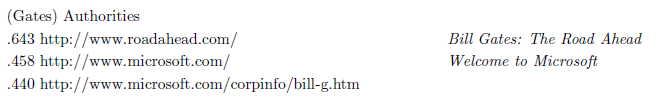
\includegraphics[scale=0.3]{gates.png} 
	\end{figure}
\end{block}
\begin{block}{www.ask.com}
	\begin{tabular}{l l}
		http://www.ask.com/wiki/Bill\_Gates?lang=en & \\
		www.gates.com/ & Gates Corporation \\
		www.gates.com/all-search-tools/automotive-interchange-search-results & Gates Corporation (manufacture)\\
		usmilitary.about.com/od/glossarytermsg/g/g2641.htm & gate \\
		www.gatesfoundation.org/ & Bill \& Melinda Gates Foundation \\
	\end{tabular}
\end{block}
\begin{block}{www.google.com}
	\begin{tabular}{l l}
		www.gates.com/ & Gates Corporation \\
		ww2.gates.com/germany/ & Gates Corporation\\
		de.wikipedia.org/wiki/Bill\_Gates & \\
		http://www.gatesbbq.com	& Gates Bar B. Q. \\
		http://www.gatesfoundation.org & Gates Foundation \\
	\end{tabular}
\end{block}

\begin{block}{www.search.yahoo.com}
	\begin{tabular}{l l}
		www.gates.com/ & Gates Corporation \\
		www.gateschevyworld.com & Gates Chevy World - Mishawaka, Elkhart, South Bend\\
		www.gatecrafters.com/design\_your\_gates.aspx & Driveway Gates | Automatic Gates | Electric Gates \\
		www.gates.com/industries/automotive & Gates Automotive Aftermarket Solutions | Gates Corporation \\
		http://www.gatesbbq.com	& Gates Bar B. Q. \\
	\end{tabular}
\end{block}

\framebreak

%\fontsize{5pt}{7.2}\selectfont

\begin{block}{HITS \cite{Kleinberg}}
	\begin{figure} [th]
		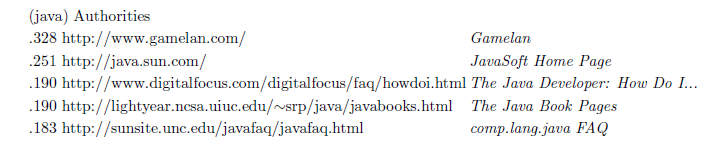
\includegraphics[scale=0.3]{java.png} 
	\end{figure}
\end{block}

\begin{block}{www.ask.com}
	\begin{tabular}{l l}
		www.ehow.com & What is Java? \\
		www.ask.com/wiki/Java\_(programming\_language)?lang=en & Wiki\\
		java.com/download & Download java\\
		java.about.com/ &  about.com\\
		www.oracle.com/technetwork/java/index.html & ORACLE\\
	\end{tabular}
\end{block}

\begin{block}{www.google.com}
	\begin{tabular}{l l}
		www.java.com/de/download/ & Download der kostenlosen Java-Software \\
		www.java.com/de/ & java.com: Java + Sie\\
		www.java.com/download & Download Free Java Software\\
		www.java.com/en/ & java.com: Java + You \\
		de.wikipedia.org/wiki/Java\_(Programmiersprache) & \\
	\end{tabular}
\end{block}

\begin{block}{www.search.yahoo.com}
	\begin{tabular}{l l}
		www.java.com & Java - Official Site \\
		java.com/en/download & Download Java \\
		www.oracle.com/technetwork/es/java/javase/overview/index.html & Java SE - Downloads \\
		windows.microsoft.com/en-US/internet-explorer/install-java & Install Java in Internet Explorer \\
		www.java.net & java.net - Official Site\\
	\end{tabular}
\end{block}

\framebreak 

%\frametitle{Ergebnisse III \cite{Kleinberg}}
\fontsize{11pt}{7.2}\selectfont
In seiner Arbeit spricht der Autor über folgende Evaluationsergebnisse:

\vspace{10pt}
Es wurden die Suchergebnisse von Yahoo!, CLEVER\footnote{Implementation von HITS mit Erweiterungen}\cite{CLEVER} und AltaVista\cite{AltaVista} verglichen, indem $37$ Freiwillige die Qualität der von verschiedenen Suchmaschinen vorgeschlagenen Seiten zu den fest gewählten Themen abschätzen sollten

\vspace{10pt}
Die Ergebnisse sind:\\
In \textcolor{maroon}{$50 \%$} der Fälle CLEVER war besser.\\
In \textcolor{maroon}{$31 \%$} Yahoo! und CLEVER waren gleich gut.\\ 
In \textcolor{maroon}{$19 \%$} Yahoo! war besser.\\ 

\end{frame}

%-------------------------------------------------------------------------------
\section{Erweiterungen des Algorithmus}

\begin{frame}
\frametitle{Suche nach ähnlichen Seiten}
\begin{itemize}
\item Die Suchanfrage $\sigma$ sei eine Internetseite\\
	\hspace{5pt} $R_\sigma = \{\text{Menge der Seiten, die auf }\sigma  \text{ zeigen}\}$
\item Wende den HITS Algorithmus an
\end{itemize}

\begin{block}{} \begin{figure}
	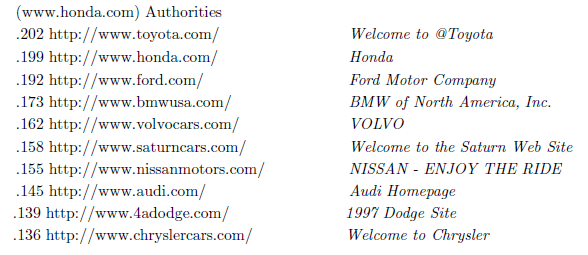
\includegraphics[scale=0.6]{honda.png}
\end{figure} \end{block}

\end{frame}


\begin{frame}
\frametitle{Mehrere Mengen von Hubs und Authorities}
\begin{itemize}
\item Der betrachtete Algorithmus liefert die am dichtesten vernetzte Menge der Authorities und Hubs im auf der Suchanfrage basierten Teilgraphen des WWWs\\
\item Es gibt eventuell weitere dicht vernetzte Mengen, die zu der Anfrage relevant sind (z.B. mehrdeutige Anfrage)
\item \textcolor{maroon}{betrachte weitere Eigenvektoren, sortiert nach Betragsgrößen}
\item
\textcolor{maroon}{betrachte positive und negative Teile eines der nicht Haupteigenvektors}
\end{itemize}

\end{frame}

%-------------------------------------------------------------------------------
\section{HITS vs PageRank}
\begin{frame}

\begin{minipage}[0.2\textheight]{\textwidth}
	\begin{columns}[T]
		\begin{column}{0.5\textwidth}
		\centering{\bf HITS}
		\begin{itemize}
			\item wird auf einem Teilgraphen des WWW angewendet
			\item einfacher, aber langsam in Echtzeit
			\item berechnet Autoritätsseiten und Hubs
			\item beruht auf textbasierter Suche
			\item kann \glqq diffundieren\grqq
		\end{itemize}
		\end{column}
		
		\begin{column}{0.5\textwidth}
		\centering{\bf PageRank}
		\begin{itemize}
			\item benutzt ganzen Graphen des WWW
			\item dauert lang, wird aber nur einmal berechnet
			\item berechnet nur Autoritätsseiten
			\item unabhängig von dem Kontext
		\end{itemize}
		\end{column}
	\end{columns}
\end{minipage}


\end{frame}

%-------------------------------------------------------------------------------


%-------------------------------------------------------------------------------
\section{Zusammenfassung}

\begin{frame}[allowframebreaks]
\frametitle{Zusammenfassung:}

\begin{itemize}
	\item Gewichtung ist sehr wichtig, besonders für breit angelegte Anfragen
	\item Als Ergebnis der Suche werden $t$ Autoritätsseiten zurückgeliefert
	\item Jeder Link enthält einen gewissen Anteil der Autorität des Erstellers des Links
	\item Autoritätsseiten sind zu der Anfrage relevante Seiten mit vielen eingehenden Links
	\item Hubs sind Seiten, die auf viele Autoritätsseiten verlinken
	\item Der ganze WWW-Graph ist zu groß $\Rightarrow$ betrachte auf der Anfrage basierten Teilgraphen
\end{itemize}

\framebreak

\begin{itemize}
\item HITS-Algorithmus
	\begin{itemize}
		\item arbeitet auf dem generierten Teilgraphen
		\item ist ein rekursiver Algorithmus
		\item konvergiert gegen Haupteigenvektoren der Matrizen $A^TA$ und $AA^T$\footnote{$A$ ist die Adjazentmatrix des betrachteten Teilgraphen}
		\item liefert Seiten zurück, die den $c$ größten Einträgen des Haupteigenvektors der Matrix $A^TA$ entsprechen
		\item kann für die Suche nach ähnlichen Seiten benutzt werden
		\item kann die für verschiedene Bedeutungen der Anfrage relevanten Seiten liefern
	\end{itemize}
\item HITS wurde in der Suchmaschine CLEVER (IBM Project) implementiert (geschlossen)
\item HITS wird in der Suchmaschine Ask.com benutzt (\cite{HITS_Lecture4_Cornell})
\end{itemize}
\end{frame}

\subsection{Modifikationen}
\begin{frame}

\frametitle{Modifikationen}
\begin{itemize}
\item Problem :\\
	\hspace{20pt} Topic Drift \\
	\hspace{20pt} Ergebnisse bei bestimmten Strukturen des Webs sind\\
	\hspace{20pt} nicht intuitiv klar \cite{Miller}
\item Modifikationen des Algorithmus
	\begin{itemize}
		\item Gewichteter HITS-Algorithmus (\cite{Bharat,Li, Miller})
		\item HITS-Algorithmus mit potenzierter Eingabe (\cite{Miller})
	\end{itemize}
\end{itemize}

\end{frame}


%-----------------------------------------------------------------------------
\begin{frame}{The End}
\centering
\LARGE
\color{red}
 Vielen Dank für Ihre Aufmerksamkeit!

 \nocite{Kleinberg}
 \nocite{ZheZhao2}
 \nocite{CIS}
 \nocite{HITS_Lecture4_Cornell}
 \nocite{BeamerTheme} 
\end{frame}

\begin{frame}
\centering
\begin{figure}
	
\includegraphics{who.png}
\end{figure}
\end{frame}

%References                                              %
\begin{frame}[allowframebreaks]
	\frametitle{References}
	\bibliographystyle{plain}
	\bibliography{bibliographie}
\end{frame} 

\end{document}
